\documentclass[11pt]{article}
\usepackage[margin=1in]{geometry}
\usepackage{amsmath,amssymb,booktabs,longtable,array,graphicx}
\usepackage[T1]{fontenc}
\setlength{\parskip}{0.4em}
\setlength{\parindent}{0pt}
\newcommand{\SEE}{\mathrm{SEE}}

\title{Saddle Escape Efficiency:\\August 2026 experimental record}
\author{Arnav Dhiman}
\date{16 August 2026}

\begin{document}
\maketitle

\section{Run}

Private script kernel, Tesla T4 GPU (\texttt{machine\_shape = NvidiaTeslaT4}).
PyTorch float64, \texttt{SEED $= 42$}. Device printed \texttt{cuda}.
Wall time $4647\,\mathrm{s}$ ($\approx 77\,\mathrm{min}$). Status: COMPLETE.

Exp.~1 $404.9\,\mathrm{s}$, exp.~2 $3419.3\,\mathrm{s}$, exp.~3 $807.7\,\mathrm{s}$.
Booth has no verified saddle and is excluded everywhere below.

Rosenbrock is not in the suite: its long curved valley is a minimizer-structure
problem, not an indefinite-saddle escape problem, so a saddle-escape score on
it is not meaningful.

\section{Method}

Escape direction: $\texttt{torch.linalg.eigh}$ on $H(x_s)$; take the column
for the smallest eigenvalue; $\ell_2$-normalize. No $2\times 2$ closed form,
no axis fallback. Dense eigh is only used in 2D. In $d\ge 10$ and on the MLP,
$\lambda_{\min},\lambda_{\max}$ come from Lanczos on Hessian-vector products
($k=\min(30,d)$, $k=25$ on the net).

Saddle search is deterministic. Candidates are sorted by gradient norm, then
lexicographically by coordinates so the same point is chosen across machines.
2D: $240\times 240$ grid, top $800$ candidates, refine with
\texttt{scipy.optimize.fsolve}. Keep a point iff
$\lVert\nabla f\rVert < 10^{-6}$, $\lambda_{\min}(H) < -10^{-4}$,
$\lambda_{\max}(H) > 10^{-4}$ (strictly indefinite, not a numerically flat
critical point). At most $3$ verified saddles per function, deduplicated by
distance $0.3$. Higher $d$: $5000$ random inits over the domain, same
lexicographic sort, at most $200$ fsolve refinements. Trajectories use the
first kept saddle.

Divergent iterates are clamped with
\texttt{nan\_to\_num}$(\cdot,\ \mathrm{nan}=\mathrm{posinf}=10^{4},\ \mathrm{neginf}=-10^{4})$
before curvature queries. The clamp is $10^{4}$ not $10^{6}$: $10^{6}$ made
Hessians ill-conditioned enough for GPU cuSOLVER \texttt{eigh} to throw.
All \texttt{eigh}/\texttt{eigvalsh} calls go through \texttt{safe\_eigh}.

\subsection{Optimizers}

GD (fixed rate); Adam $(0.9,0.999)$, $\varepsilon=10^{-8}$;
RMSProp $\alpha=0.99$, $\varepsilon=10^{-8}$;
AdaGrad $\varepsilon=10^{-8}$ (set explicitly; PyTorch default is $10^{-10}$);
AdamW $\mathrm{weight\_decay}=0.01$;
SGD momentum $0.9$.

\subsection{Escape criteria (evaluated on the same trajectories)}

\begin{align*}
\text{A: } &\lVert x_t-x_s\rVert > r, && r\in\{1.5,2.0,3.0\},\\
\text{B: } &\lambda_{\min}(H(x_t)) > -\varepsilon, && \varepsilon\in\{10^{-2},10^{-3},10^{-4}\},\\
\text{C: } &\lvert\langle x_t-x_s,v\rangle\rvert > c\,r_{\mathrm{curv}}, &&
  c\in\{0.5,1.0,2.0\},\quad r_{\mathrm{curv}}=1/\sqrt{\lvert\lambda_{\min}\rvert},\\
\text{D: } &f(x_t)<f(x_s)-\delta \ \text{and}\ \lambda_{\min}(H(x_t))>-10^{-3}, &&
  \delta\in\{0.25,0.5,1.0\}.
\end{align*}
Headline parameters: $r=2$, $\varepsilon=10^{-3}$, $c=1$, $\delta=0.5$.
Criterion C uses $r_{\mathrm{curv}}$ because that is the natural length of
the unstable manifold at a quadratic saddle; a fixed radius is the wrong
scale when $|\lambda_{\min}|$ spans two orders of magnitude.

\subsection{SEE}

\[
\SEE = P_{\mathrm{esc}}/\overline{\tau}_{\mathrm{esc}},
\]
with $\overline{\tau}_{\mathrm{esc}}$ the mean first hitting time among
escaped trials (uncensored at $T_{\max}$). Bootstrap $95\%$ CIs, $B=2000$
resamples, reported as asymmetric percentile intervals $[lo,hi]$, not
symmetric $\pm$. Init: $x_0 = x_s + 0.1\,\mathcal{N}(0,I)$.

\section{Experiment 1: 2D benchmarks}

Eight functions, all six optimizers, all four criteria.
LR sweep $\{0.001,0.01,0.05,0.1,0.2,0.5\}$, $N=200$, $T_{\max}=200$.
Domains: Himmelblau $[-6,6]^2$, Ackley $[-5,5]^2$, Rastrigin $[-5.12,5.12]^2$,
Styblinski $[-5,5]^2$, Levy $[-8,8]^2$, Beale $[-4.5,4.5]^2$,
Booth $[-10,10]^2$, Schwefel $[-500,500]^2$.

\subsection{Verified saddles}

\begin{center}
\begin{tabular}{lcccr}
\toprule
Function & $n$ saddles & $x_s$ & $\lambda_{\min}$ & $r_{\mathrm{curv}}$ \\
\midrule
Himmelblau & 3 & $(-0.128,-1.954)$ & $-50.61$ & $0.141$ \\
Ackley     & 3 & $(-0.577,\ 0.875)$ & $-17.11$ & $0.242$ \\
Rastrigin  & 3 & $(-0.503,\ 0.000)$ & $-392.73$ & $0.050$ \\
Styblinski & 3 & $(0.157,\ 2.747)$ & $-15.85$ & $0.251$ \\
Levy       & 3 & $(1.000,-2.257)$ & $-2.96$ & $0.582$ \\
Beale      & 2 & $(0.000,\ 1.000)$ & $-27.75$ & $0.190$ \\
Booth      & 0 & -- & -- & -- \\
Schwefel   & 3 & $(-5.239,\ 5.239)$ & $-0.40$ & $1.574$ \\
\bottomrule
\end{tabular}
\end{center}

\subsection{Best-LR SEE (headline parameter of each family)}

\begin{center}
\small
\begin{tabular}{llcccc}
\toprule
Function & Opt. & A & B & C & D \\
\midrule
Himmelblau & GD      & $0.637$ & $0.543$ & $0.943$ & $0.227$ \\
           & Adam    & $0.216$ & $0.143$ & $1.000$ & $0.143$ \\
           & RMSProp & $1.000$ & $1.000$ & $1.000$ & $0.451$ \\
           & AdaGrad & $0.210$ & $0.199$ & $1.000$ & $0.199$ \\
           & AdamW   & $0.213$ & $0.140$ & $1.000$ & $0.140$ \\
           & SGD\_mom& $0.639$ & $0.542$ & $0.943$ & $0.207$ \\
\midrule
Ackley     & GD      & $0.305$ & $0.254$ & $0.758$ & $0.251$ \\
           & Adam    & $0.000$ & $0.342$ & $1.000$ & $0.333$ \\
           & RMSProp & $1.000$ & $0.286$ & $1.000$ & $0.286$ \\
           & AdaGrad & $0.000$ & $0.437$ & $1.000$ & $0.426$ \\
           & AdamW   & $0.001$ & $0.338$ & $1.000$ & $0.329$ \\
           & SGD\_mom& $0.359$ & $0.186$ & $0.755$ & $0.181$ \\
\midrule
Rastrigin  & GD      & $0.985$ & $0.303$ & $0.990$ & $0.303$ \\
           & Adam    & $0.000$ & $0.709$ & $1.000$ & $0.709$ \\
           & RMSProp & $1.000$ & $0.421$ & $1.000$ & $0.421$ \\
           & AdaGrad & $0.000$ & $0.709$ & $1.000$ & $0.709$ \\
           & AdamW   & $0.000$ & $0.709$ & $1.000$ & $0.709$ \\
           & SGD\_mom& $0.985$ & $0.299$ & $0.990$ & $0.239$ \\
\midrule
Styblinski & GD      & $0.549$ & $0.444$ & $0.749$ & $0.221$ \\
           & Adam    & $0.208$ & $0.252$ & $1.000$ & $0.252$ \\
           & RMSProp & $1.000$ & $1.000$ & $1.000$ & $0.500$ \\
           & AdaGrad & $0.200$ & $0.267$ & $1.000$ & $0.267$ \\
           & AdamW   & $0.207$ & $0.249$ & $1.000$ & $0.249$ \\
           & SGD\_mom& $0.548$ & $0.442$ & $0.749$ & $0.230$ \\
\midrule
Levy       & GD      & $0.017$ & $0.332$ & $0.291$ & $0.147$ \\
           & Adam    & $0.103$ & $0.746$ & $0.610$ & $0.255$ \\
           & RMSProp & $1.000$ & $0.746$ & $1.000$ & $0.255$ \\
           & AdaGrad & $0.013$ & $0.746$ & $0.610$ & $0.255$ \\
           & AdamW   & $0.104$ & $0.763$ & $0.613$ & $0.255$ \\
           & SGD\_mom& $0.112$ & $0.366$ & $0.330$ & $0.160$ \\
\midrule
Beale      & GD      & $0.585$ & $0.230$ & $0.897$ & $0.228$ \\
           & Adam    & $0.028$ & $0.208$ & $0.377$ & $0.208$ \\
           & RMSProp & $1.000$ & $0.213$ & $0.350$ & $0.213$ \\
           & AdaGrad & $0.037$ & $0.212$ & $0.372$ & $0.212$ \\
           & AdamW   & $0.027$ & $0.216$ & $0.372$ & $0.216$ \\
           & SGD\_mom& $0.587$ & $0.244$ & $0.897$ & $0.244$ \\
\midrule
Schwefel   & GD      & $0.047$ & $0.035$ & $0.050$ & $0.035$ \\
           & Adam    & $0.207$ & $0.072$ & $0.256$ & $0.072$ \\
           & RMSProp & $1.000$ & $0.565$ & $1.000$ & $0.500$ \\
           & AdaGrad & $0.200$ & $0.029$ & $0.258$ & $0.029$ \\
           & AdamW   & $0.207$ & $0.068$ & $0.254$ & $0.068$ \\
           & SGD\_mom& $0.092$ & $0.073$ & $0.097$ & $0.073$ \\
\bottomrule
\end{tabular}
\end{center}

\subsection{Pairwise Spearman $\rho$ of best-LR SEE ranks}

\begin{center}
\small
\begin{tabular}{lcccccc}
\toprule
Function & A-B & A-C & A-D & B-C & B-D & C-D \\
\midrule
Himmelblau & $+0.77$ & $-0.41$ & $+0.77$ & $-0.41$ & $+1.00$ & $-0.41$ \\
Ackley     & $-0.81$ & $-0.45$ & $-0.81$ & $+0.85$ & $+1.00$ & $+0.85$ \\
Rastrigin  & $-0.79$ & $-0.45$ & $-0.79$ & $+0.88$ & $+1.00$ & $+0.88$ \\
Styblinski & $+0.83$ & $-0.41$ & $-0.09$ & $-0.41$ & $+0.09$ & $+0.83$ \\
Levy       & $+0.15$ & $+0.49$ & $+0.10$ & $+0.83$ & $+0.90$ & $+0.86$ \\
Beale      & $+0.37$ & $0.00$  & $+0.37$ & $+0.53$ & $+1.00$ & $+0.53$ \\
Schwefel   & $+0.49$ & $+0.77$ & $+0.49$ & $+0.26$ & $+1.00$ & $+0.26$ \\
\bottomrule
\end{tabular}
\end{center}

B and D agree almost perfectly ($\rho=1$ on five of seven functions): D's
curvature clause is essentially B with an extra loss-drop filter.

\subsection{Kendall's $W$ across A,B,C,D}

\begin{center}
\begin{tabular}{lcr}
\toprule
Function & $W$ & $\lambda_{\min}$ \\
\midrule
Himmelblau & $0.420$ & $-50.61$ \\
Ackley     & $0.288$ & $-17.11$ \\
Rastrigin  & $0.275$ & $-392.73$ \\
Styblinski & $0.334$ & $-15.85$ \\
Levy       & $0.588$ & $-2.96$ \\
Beale      & $0.593$ & $-27.75$ \\
Schwefel   & $0.657$ & $-0.40$ \\
\bottomrule
\end{tabular}
\end{center}

\subsection{Within-family stability}

Spearman $\rho$ between the extreme parameter of each family
(A: $r=1.5$ vs $3.0$; B: $\varepsilon=10^{-2}$ vs $10^{-4}$;
C: $c=0.5$ vs $2.0$; D: $\delta=0.25$ vs $1.0$).

\begin{center}
\begin{tabular}{lcccc}
\toprule
Function & A & B & C & D \\
\midrule
Himmelblau & $0.82$ & $1.00$ & $1.00$ & $1.00$ \\
Ackley     & $0.94$ & $1.00$ & $-0.41$ & $0.77$ \\
Rastrigin  & $1.00$ & $1.00$ & $1.00$ & $1.00$ \\
Styblinski & $0.81$ & $1.00$ & $0.90$ & $1.00$ \\
Levy       & $0.83$ & $1.00$ & $0.86$ & $0.28$ \\
Beale      & $0.99$ & $1.00$ & $0.81$ & $1.00$ \\
Schwefel   & $0.77$ & $1.00$ & $0.94$ & $1.00$ \\
\bottomrule
\end{tabular}
\end{center}
B is invariant to its $\varepsilon$ on every function. C is unstable only on
Ackley ($\rho=-0.41$). D is unstable only on Levy ($\rho=0.28$).

\section{Experiment 2: higher dimension}

Rastrigin and Ackley at $d=10,50$. Criteria A and B only.
$N=100$, $T_{\max}=500$, same LR sweep. 2D $\rho(A,B)$ from exp.~1 is the
anchor.

\subsection{Saddles}

\begin{center}
\begin{tabular}{lcc}
\toprule
 & $d$ & $\lambda_{\min}$ \\
\midrule
Rastrigin & 10 & $-391.52$ \\
Rastrigin & 50 & $-392.73$ \\
Ackley    & 10 & $-3.96$ \\
Ackley    & 50 & $-0.70$ \\
\bottomrule
\end{tabular}
\end{center}
Three verified saddles in each case.

\subsection{Best-LR SEE}

\begin{center}
\small
\begin{tabular}{llccc}
\toprule
Function & Opt. & $d$ & A & B \\
\midrule
Rastrigin & GD      & 10 & $1.000$ & $0.184$ \\
          & Adam    & 10 & $0.095$ & $0.714$ \\
          & RMSProp & 10 & $1.000$ & $0.426$ \\
          & AdaGrad & 10 & $0.016$ & $0.714$ \\
          & AdamW   & 10 & $0.145$ & $0.719$ \\
          & SGD\_mom& 10 & $1.000$ & $0.263$ \\
\midrule
Rastrigin & GD      & 50 & $1.000$ & $0.069$ \\
          & Adam    & 50 & $1.000$ & $0.500$ \\
          & RMSProp & 50 & $1.000$ & $0.333$ \\
          & AdaGrad & 50 & $1.000$ & $0.500$ \\
          & AdamW   & 50 & $1.000$ & $0.500$ \\
          & SGD\_mom& 50 & $1.000$ & $0.078$ \\
\midrule
Ackley    & GD      & 10 & $0.084$ & $0.206$ \\
          & Adam    & 10 & $0.376$ & $0.424$ \\
          & RMSProp & 10 & $1.000$ & $0.249$ \\
          & AdaGrad & 10 & $0.197$ & $0.455$ \\
          & AdamW   & 10 & $0.389$ & $0.427$ \\
          & SGD\_mom& 10 & $0.247$ & $0.107$ \\
\midrule
Ackley    & GD      & 50 & $0.148$ & $0.095$ \\
          & Adam    & 50 & $1.000$ & $0.369$ \\
          & RMSProp & 50 & $1.000$ & $0.221$ \\
          & AdaGrad & 50 & $1.000$ & $0.441$ \\
          & AdamW   & 50 & $1.000$ & $0.379$ \\
          & SGD\_mom& 50 & $0.239$ & $0.048$ \\
\bottomrule
\end{tabular}
\end{center}

\subsection{$\rho(A,B)$ vs dimension}

\begin{center}
\begin{tabular}{lccc}
\toprule
 & $d=2$ & $d=10$ & $d=50$ \\
\midrule
Rastrigin & $-0.79$ & $-0.74$ & -- \\
Ackley    & $-0.81$ & $+0.14$ & $+0.78$ \\
\bottomrule
\end{tabular}
\end{center}
Rastrigin $d=50$ is undefined: every optimizer has $\mathrm{best}_A=1$, so
Spearman sees a constant. A saturates; B still separates
Adam/AdaGrad/AdamW from GD/SGD\_mom.

\section{Experiment 3: XOR MLP}

Architecture: input $2$, hidden $8$, output $1$, $\tanh$, no hidden bias
($D=25$ flattened parameters). XOR replicated to $200$ samples, Gaussian
noise $\sigma=0.05$, MSE. Saddles in parameter space: random inits + fsolve,
accept indefinite parameter Hessians. Criteria A,B only. $N=50$,
$T_{\max}=300$, LR $\{0.001,0.005,0.01,0.05,0.1\}$.

Two saddles found. Used saddle: $\mathrm{loss}=0.173$,
$\lambda_{\min}=-0.402$, $\lambda_{\max}=7.646$.

\begin{center}
\begin{tabular}{lcc}
\toprule
Opt. & A & B \\
\midrule
GD      & $0.000$ & $0.000$ \\
Adam    & $0.091$ & $0.010$ \\
RMSProp & $1.000$ & $0.006$ \\
AdaGrad & $0.044$ & $0.005$ \\
AdamW   & $0.092$ & $0.010$ \\
SGD\_mom& $0.006$ & $0.000$ \\
\bottomrule
\end{tabular}
\end{center}
$\rho(A,B)=+0.81$. No rank inversion. RMSProp dominates distance; curvature
escape is near zero for all six.

\section{Curvature-sharpness}

Spearman correlation of $|\lambda_{\min}|$ with Kendall's $W$ on the original
five functions (Himmelblau, Ackley, Rastrigin, Styblinski, Levy). Exact
two-sided $p$-value by enumerating all $5!=120$ permutations of $W$.

\[
\rho\bigl(|\lambda_{\min}|,\,W\bigr) = -0.7,\qquad p = 0.2333,\quad n=5.
\]
Sharper saddles go with less criterion agreement. Not significant at $n=5$.

\section{Answers to the preset questions}

\paragraph{Does the A-vs-B inversion persist in 10D, 50D, and on the net?}
On Rastrigin 10D, yes ($\rho=-0.74$). On Rastrigin 50D the coefficient is
undefined because A saturates. On Ackley it \emph{disappears} with dimension
($-0.81\to +0.14\to +0.78$). On the XOR-MLP, $\rho=+0.81$: no inversion.

\paragraph{Where do AdamW and SGD+momentum rank under B versus A?}
AdamW: mean $\mathrm{best}_A=0.108$ (typically $4$-$6/6$),
mean $\mathrm{best}_B=0.355$, and $1/6$ on Rastrigin and Levy under B.
SGD\_mom: mean $\mathrm{best}_A=0.475$ (typically $2/6$),
mean $\mathrm{best}_B=0.307$, and $6/6$ on Ackley and Rastrigin under B.

\begin{center}
\small
\begin{tabular}{lcccc}
\toprule
Function & AdamW $r_A$ & AdamW $r_B$ & SGD\_mom $r_A$ & SGD\_mom $r_B$ \\
\midrule
Himmelblau & $5/6$ & $6/6$ & $2/6$ & $3/6$ \\
Ackley     & $4/6$ & $3/6$ & $2/6$ & $6/6$ \\
Rastrigin  & $4/6$ & $1/6$ & $2/6$ & $6/6$ \\
Styblinski & $5/6$ & $6/6$ & $3/6$ & $3/6$ \\
Levy       & $3/6$ & $1/6$ & $2/6$ & $5/6$ \\
Beale      & $6/6$ & $3/6$ & $2/6$ & $1/6$ \\
Schwefel   & $2/6$ & $4/6$ & $5/6$ & $2/6$ \\
\bottomrule
\end{tabular}
\end{center}

\paragraph{Does C still saturate?}
On Himmelblau, Ackley, Rastrigin, Styblinski: yes ($4/6$ optimizers at $1.0$).
It discriminates on Levy $[0.291,1.000]$ ($1/6$ at $1.0$),
Beale $[0.350,0.897]$ ($0/6$ at $1.0$),
Schwefel $[0.050,1.000]$ ($1/6$ at $1.0$).

\paragraph{Curvature-sharpness?}
$\rho=-0.7$, exact $p=0.2333$, $n=5$.

\paragraph{Do the three new functions match the original five?}
Booth: no saddle, excluded. Beale $\rho(A,B)=+0.37$, $W=0.593$.
Schwefel $\rho(A,B)=+0.49$, $W=0.657$.
They follow Himmelblau/Styblinski (positive A-B), not Ackley/Rastrigin
(inversion). C is less saturated on the new functions than on the original
sharp 2D set. RMSProp still dominates A.

\section{Headline $\mathrm{LR}=0.2$ SEE with $95\%$ bootstrap CIs}

Not best-LR; this is the single-LR slice. Intervals are percentile $[2.5,97.5]$.

{\small
\begin{longtable}{llcccc}
\toprule
Function & Opt. & A & B & C & D \\
\midrule
\endfirsthead
\toprule
Function & Opt. & A & B & C & D \\
\midrule
\endhead
Himmelblau & GD & $0.485\ [0.471,0.501]$ & $0.435\ [0.418,0.452]$ & $0.877\ [0.833,0.917]$ & $0.103\ [0.073,0.134]$ \\
 & Adam & $0.102\ [0.102,0.103]$ & $0.065\ [0.062,0.068]$ & $1.000\ [1.000,1.000]$ & $0.065\ [0.062,0.068]$ \\
 & RMSProp & $1.000\ [1.000,1.000]$ & $0.451\ [0.437,0.468]$ & $1.000\ [1.000,1.000]$ & $0.451\ [0.436,0.466]$ \\
 & AdaGrad & $0.062\ [0.062,0.062]$ & $0.050\ [0.049,0.050]$ & $1.000\ [1.000,1.000]$ & $0.050\ [0.049,0.050]$ \\
 & AdamW & $0.102\ [0.101,0.102]$ & $0.063\ [0.061,0.067]$ & $1.000\ [1.000,1.000]$ & $0.063\ [0.061,0.067]$ \\
 & SGD\_mom & $0.485\ [0.469,0.503]$ & $0.448\ [0.433,0.465]$ & $0.877\ [0.837,0.917]$ & $0.105\ [0.075,0.136]$ \\
Ackley & GD & $0.076\ [0.070,0.084]$ & $0.128\ [0.114,0.146]$ & $0.595\ [0.554,0.639]$ & $0.115\ [0.102,0.129]$ \\
 & Adam & $0.000\ [0.000,0.000]$ & $0.342\ [0.316,0.375]$ & $0.746\ [0.712,0.784]$ & $0.333\ [0.309,0.362]$ \\
 & RMSProp & $1.000\ [1.000,1.000]$ & $0.095\ [0.087,0.106]$ & $1.000\ [1.000,1.000]$ & $0.047\ [0.041,0.053]$ \\
 & AdaGrad & $0.000\ [0.000,0.000]$ & $0.437\ [0.413,0.465]$ & $0.746\ [0.709,0.784]$ & $0.426\ [0.403,0.448]$ \\
 & AdamW & $0.000\ [0.000,0.000]$ & $0.338\ [0.312,0.371]$ & $0.743\ [0.707,0.778]$ & $0.329\ [0.305,0.357]$ \\
 & SGD\_mom & $0.191\ [0.178,0.204]$ & $0.143\ [0.124,0.166]$ & $0.602\ [0.563,0.647]$ & $0.059\ [0.039,0.093]$ \\
Rastrigin & GD & $0.957\ [0.930,0.980]$ & $0.247\ [0.220,0.280]$ & $0.971\ [0.948,0.990]$ & $0.011\ [0.010,0.013]$ \\
 & Adam & $0.000\ [0.000,0.000]$ & $0.709\ [0.678,0.746]$ & $1.000\ [1.000,1.000]$ & $0.709\ [0.676,0.746]$ \\
 & RMSProp & $1.000\ [1.000,1.000]$ & $0.255\ [0.224,0.293]$ & $1.000\ [1.000,1.000]$ & $0.049\ [0.041,0.058]$ \\
 & AdaGrad & $0.000\ [0.000,0.000]$ & $0.709\ [0.676,0.743]$ & $1.000\ [1.000,1.000]$ & $0.709\ [0.676,0.746]$ \\
 & AdamW & $0.000\ [0.000,0.000]$ & $0.709\ [0.678,0.743]$ & $1.000\ [1.000,1.000]$ & $0.709\ [0.676,0.743]$ \\
 & SGD\_mom & $0.957\ [0.930,0.980]$ & $0.249\ [0.222,0.282]$ & $0.971\ [0.948,0.990]$ & $0.003\ [0.002,0.004]$ \\
Styblinski & GD & $0.384\ [0.371,0.398]$ & $0.306\ [0.293,0.320]$ & $0.563\ [0.525,0.606]$ & $0.098\ [0.075,0.124]$ \\
 & Adam & $0.095\ [0.094,0.095]$ & $0.114\ [0.112,0.116]$ & $0.697\ [0.664,0.730]$ & $0.114\ [0.112,0.116]$ \\
 & RMSProp & $1.000\ [1.000,1.000]$ & $0.662\ [0.633,0.694]$ & $1.000\ [1.000,1.000]$ & $0.402\ [0.391,0.414]$ \\
 & AdaGrad & $0.052\ [0.052,0.052]$ & $0.077\ [0.075,0.078]$ & $0.697\ [0.664,0.733]$ & $0.077\ [0.075,0.078]$ \\
 & AdamW & $0.094\ [0.093,0.095]$ & $0.113\ [0.111,0.114]$ & $0.697\ [0.664,0.733]$ & $0.113\ [0.111,0.115]$ \\
 & SGD\_mom & $0.382\ [0.368,0.394]$ & $0.322\ [0.308,0.338]$ & $0.578\ [0.541,0.619]$ & $0.154\ [0.126,0.183]$ \\
Levy & GD & $0.007\ [0.006,0.008]$ & $0.179\ [0.168,0.191]$ & $0.149\ [0.142,0.157]$ & $0.079\ [0.068,0.093]$ \\
 & Adam & $0.042\ [0.037,0.048]$ & $0.388\ [0.371,0.407]$ & $0.310\ [0.303,0.317]$ & $0.141\ [0.121,0.160]$ \\
 & RMSProp & $1.000\ [1.000,1.000]$ & $0.241\ [0.221,0.263]$ & $1.000\ [1.000,1.000]$ & $0.107\ [0.081,0.138]$ \\
 & AdaGrad & $0.003\ [0.002,0.003]$ & $0.396\ [0.380,0.414]$ & $0.304\ [0.299,0.311]$ & $0.139\ [0.120,0.156]$ \\
 & AdamW & $0.043\ [0.037,0.049]$ & $0.390\ [0.372,0.410]$ & $0.308\ [0.301,0.315]$ & $0.143\ [0.124,0.163]$ \\
 & SGD\_mom & $0.070\ [0.060,0.080]$ & $0.242\ [0.229,0.256]$ & $0.217\ [0.207,0.228]$ & $0.108\ [0.091,0.125]$ \\
Beale & GD & $0.426\ [0.412,0.440]$ & $0.204\ [0.164,0.244]$ & $0.752\ [0.709,0.797]$ & $0.201\ [0.161,0.243]$ \\
 & Adam & $0.017\ [0.015,0.019]$ & $0.196\ [0.182,0.211]$ & $0.377\ [0.339,0.422]$ & $0.196\ [0.183,0.212]$ \\
 & RMSProp & $1.000\ [1.000,1.000]$ & $0.014\ [0.012,0.016]$ & $0.036\ [0.029,0.048]$ & $0.014\ [0.012,0.016]$ \\
 & AdaGrad & $0.014\ [0.011,0.016]$ & $0.192\ [0.180,0.207]$ & $0.372\ [0.335,0.418]$ & $0.192\ [0.180,0.208]$ \\
 & AdamW & $0.016\ [0.015,0.018]$ & $0.194\ [0.180,0.209]$ & $0.372\ [0.334,0.418]$ & $0.194\ [0.180,0.210]$ \\
 & SGD\_mom & $0.426\ [0.412,0.441]$ & $0.207\ [0.166,0.250]$ & $0.755\ [0.714,0.797]$ & $0.201\ [0.160,0.246]$ \\
Schwefel & GD & $0.020\ [0.019,0.021]$ & $0.015\ [0.014,0.016]$ & $0.021\ [0.020,0.023]$ & $0.015\ [0.014,0.016]$ \\
 & Adam & $0.094\ [0.094,0.095]$ & $0.033\ [0.031,0.035]$ & $0.117\ [0.116,0.118]$ & $0.033\ [0.031,0.035]$ \\
 & RMSProp & $1.000\ [1.000,1.000]$ & $0.246\ [0.230,0.265]$ & $1.000\ [1.000,1.000]$ & $0.246\ [0.230,0.265]$ \\
 & AdaGrad & $0.059\ [0.059,0.059]$ & $0.009\ [0.008,0.010]$ & $0.085\ [0.085,0.086]$ & $0.009\ [0.008,0.010]$ \\
 & AdamW & $0.093\ [0.092,0.094]$ & $0.031\ [0.030,0.033]$ & $0.117\ [0.115,0.118]$ & $0.031\ [0.030,0.033]$ \\
 & SGD\_mom & $0.056\ [0.053,0.058]$ & $0.044\ [0.042,0.045]$ & $0.059\ [0.056,0.061]$ & $0.044\ [0.042,0.046]$ \\
\bottomrule
\end{longtable}
}

\section{Figures}

Figures live in \texttt{results/} (compile this file from \texttt{writeup/}).

\begin{figure}[ht]\centering
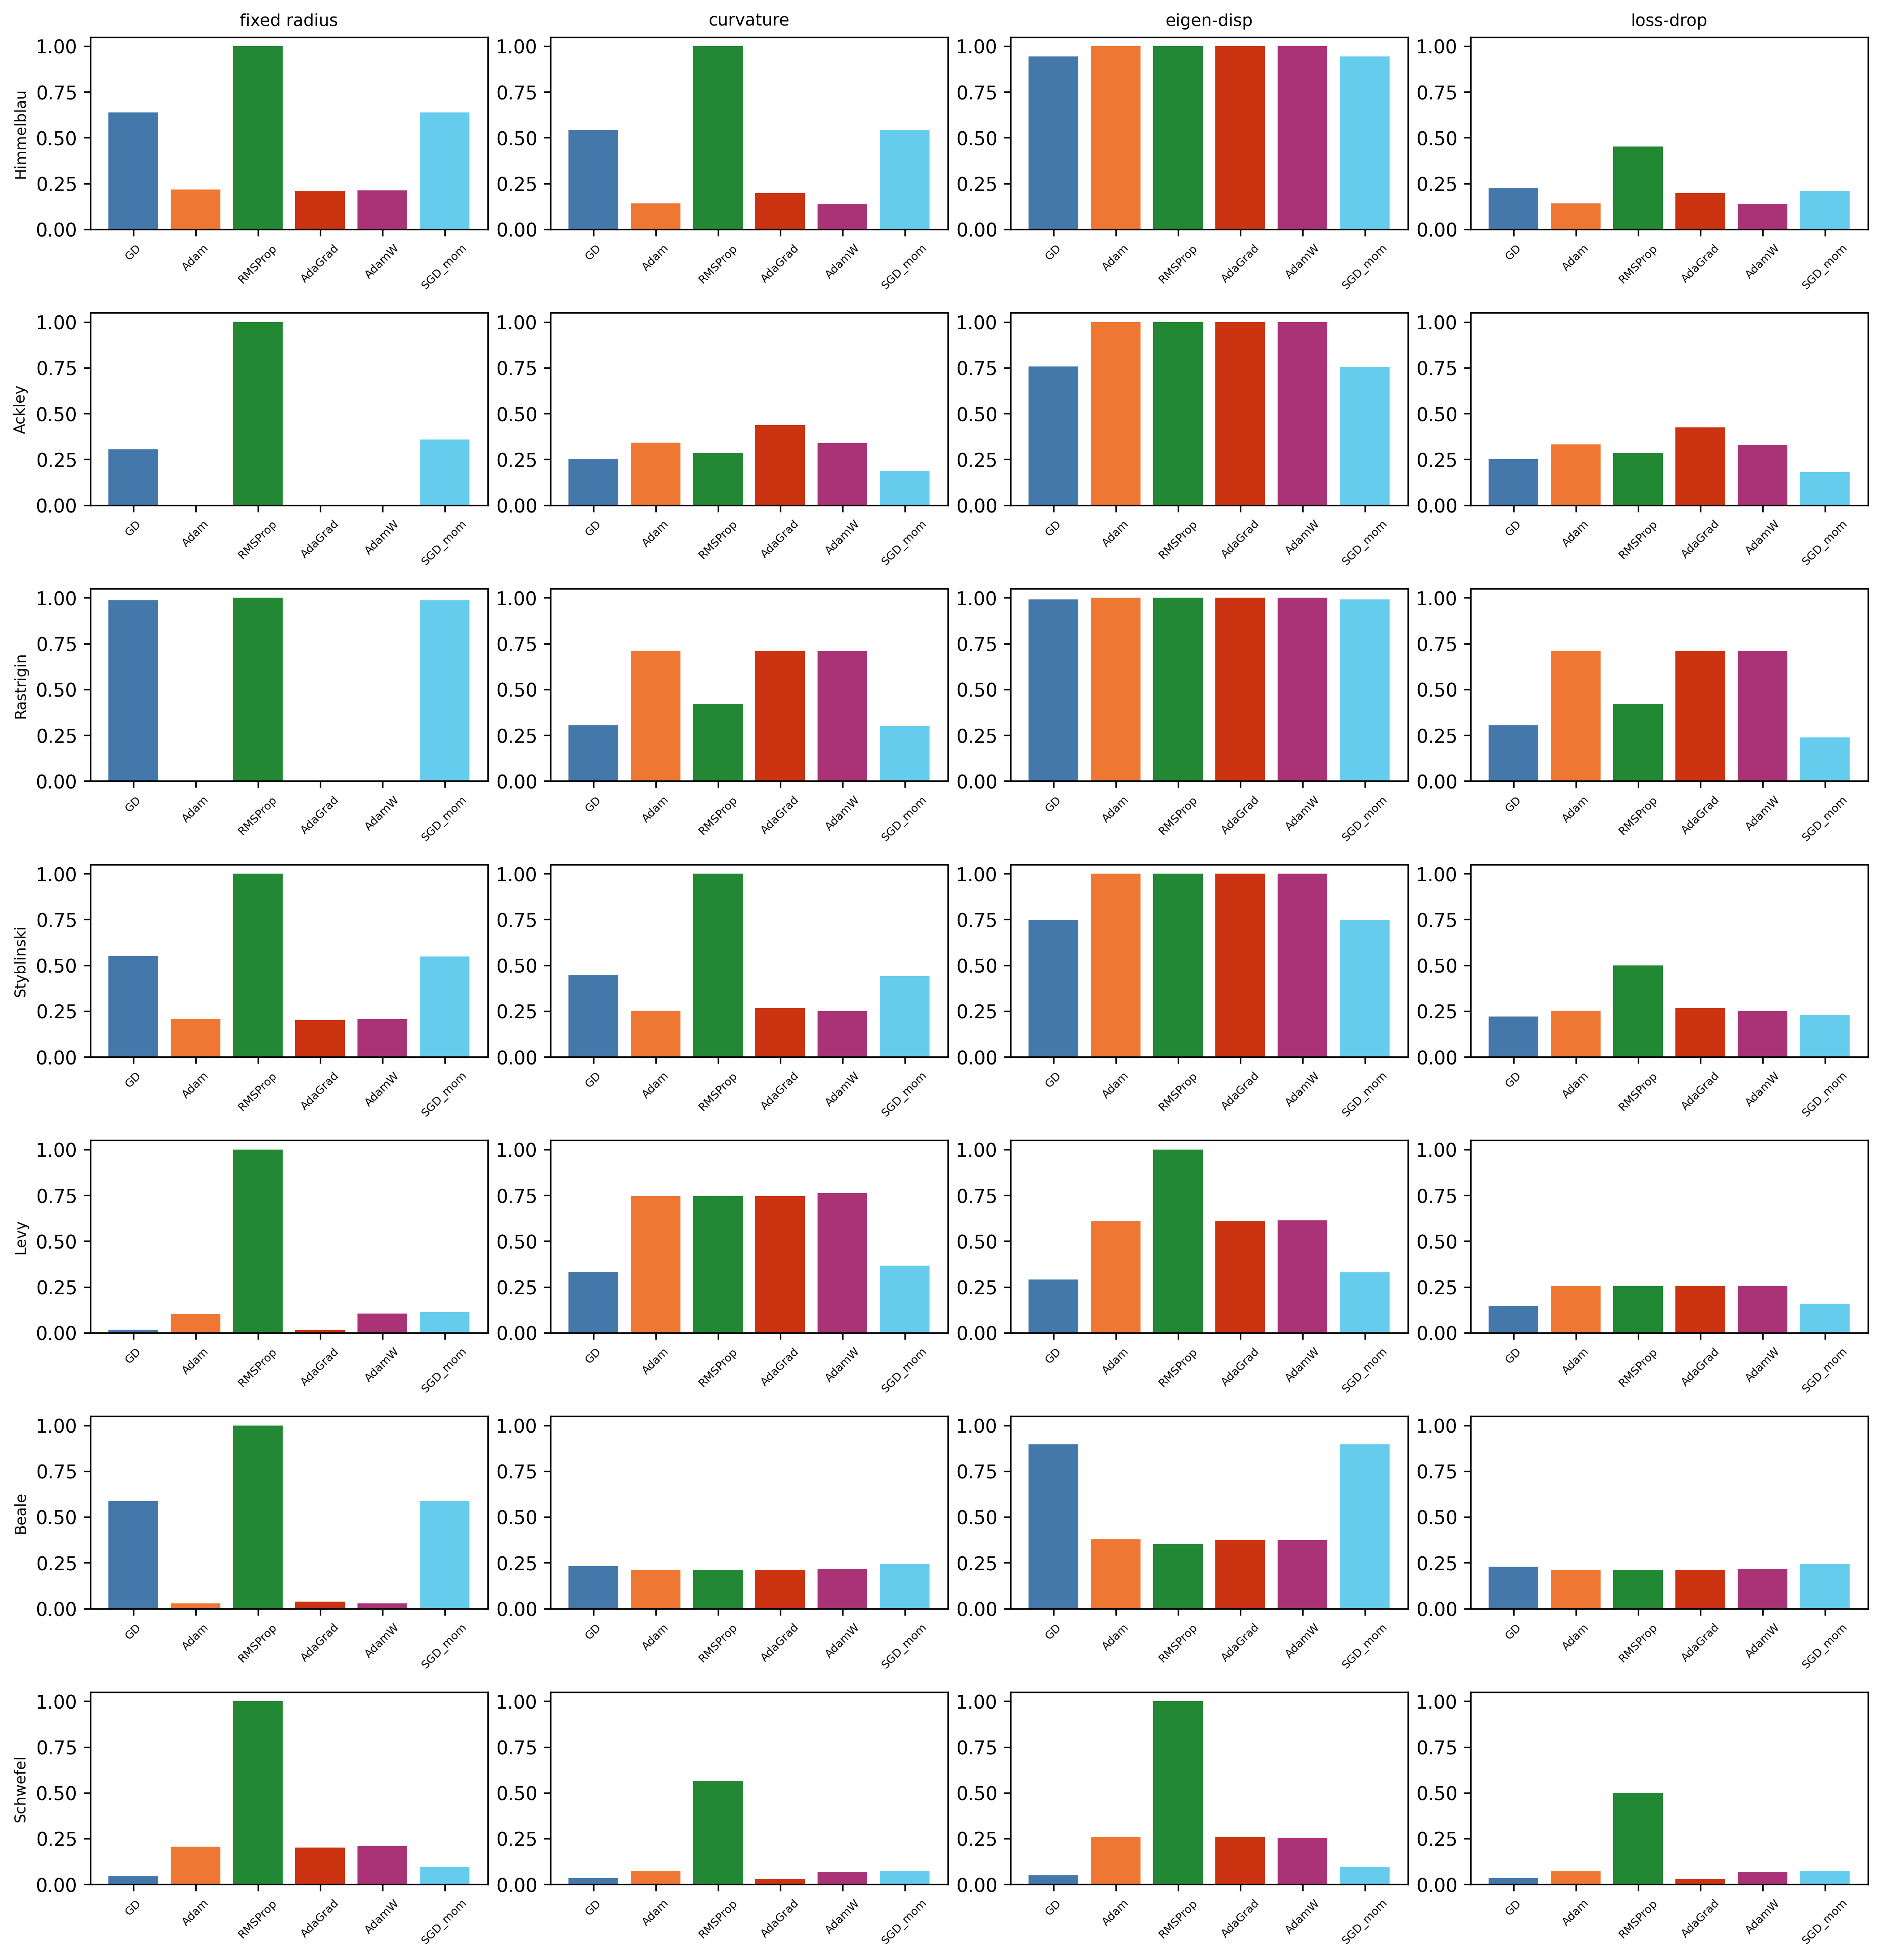
\includegraphics[width=\textwidth]{../results/1_two_dimensional/figures/fig1_criteria_grid.png}
\caption{Best-LR SEE, all 2D functions $\times$ four criteria.}
\end{figure}

\begin{figure}[ht]\centering
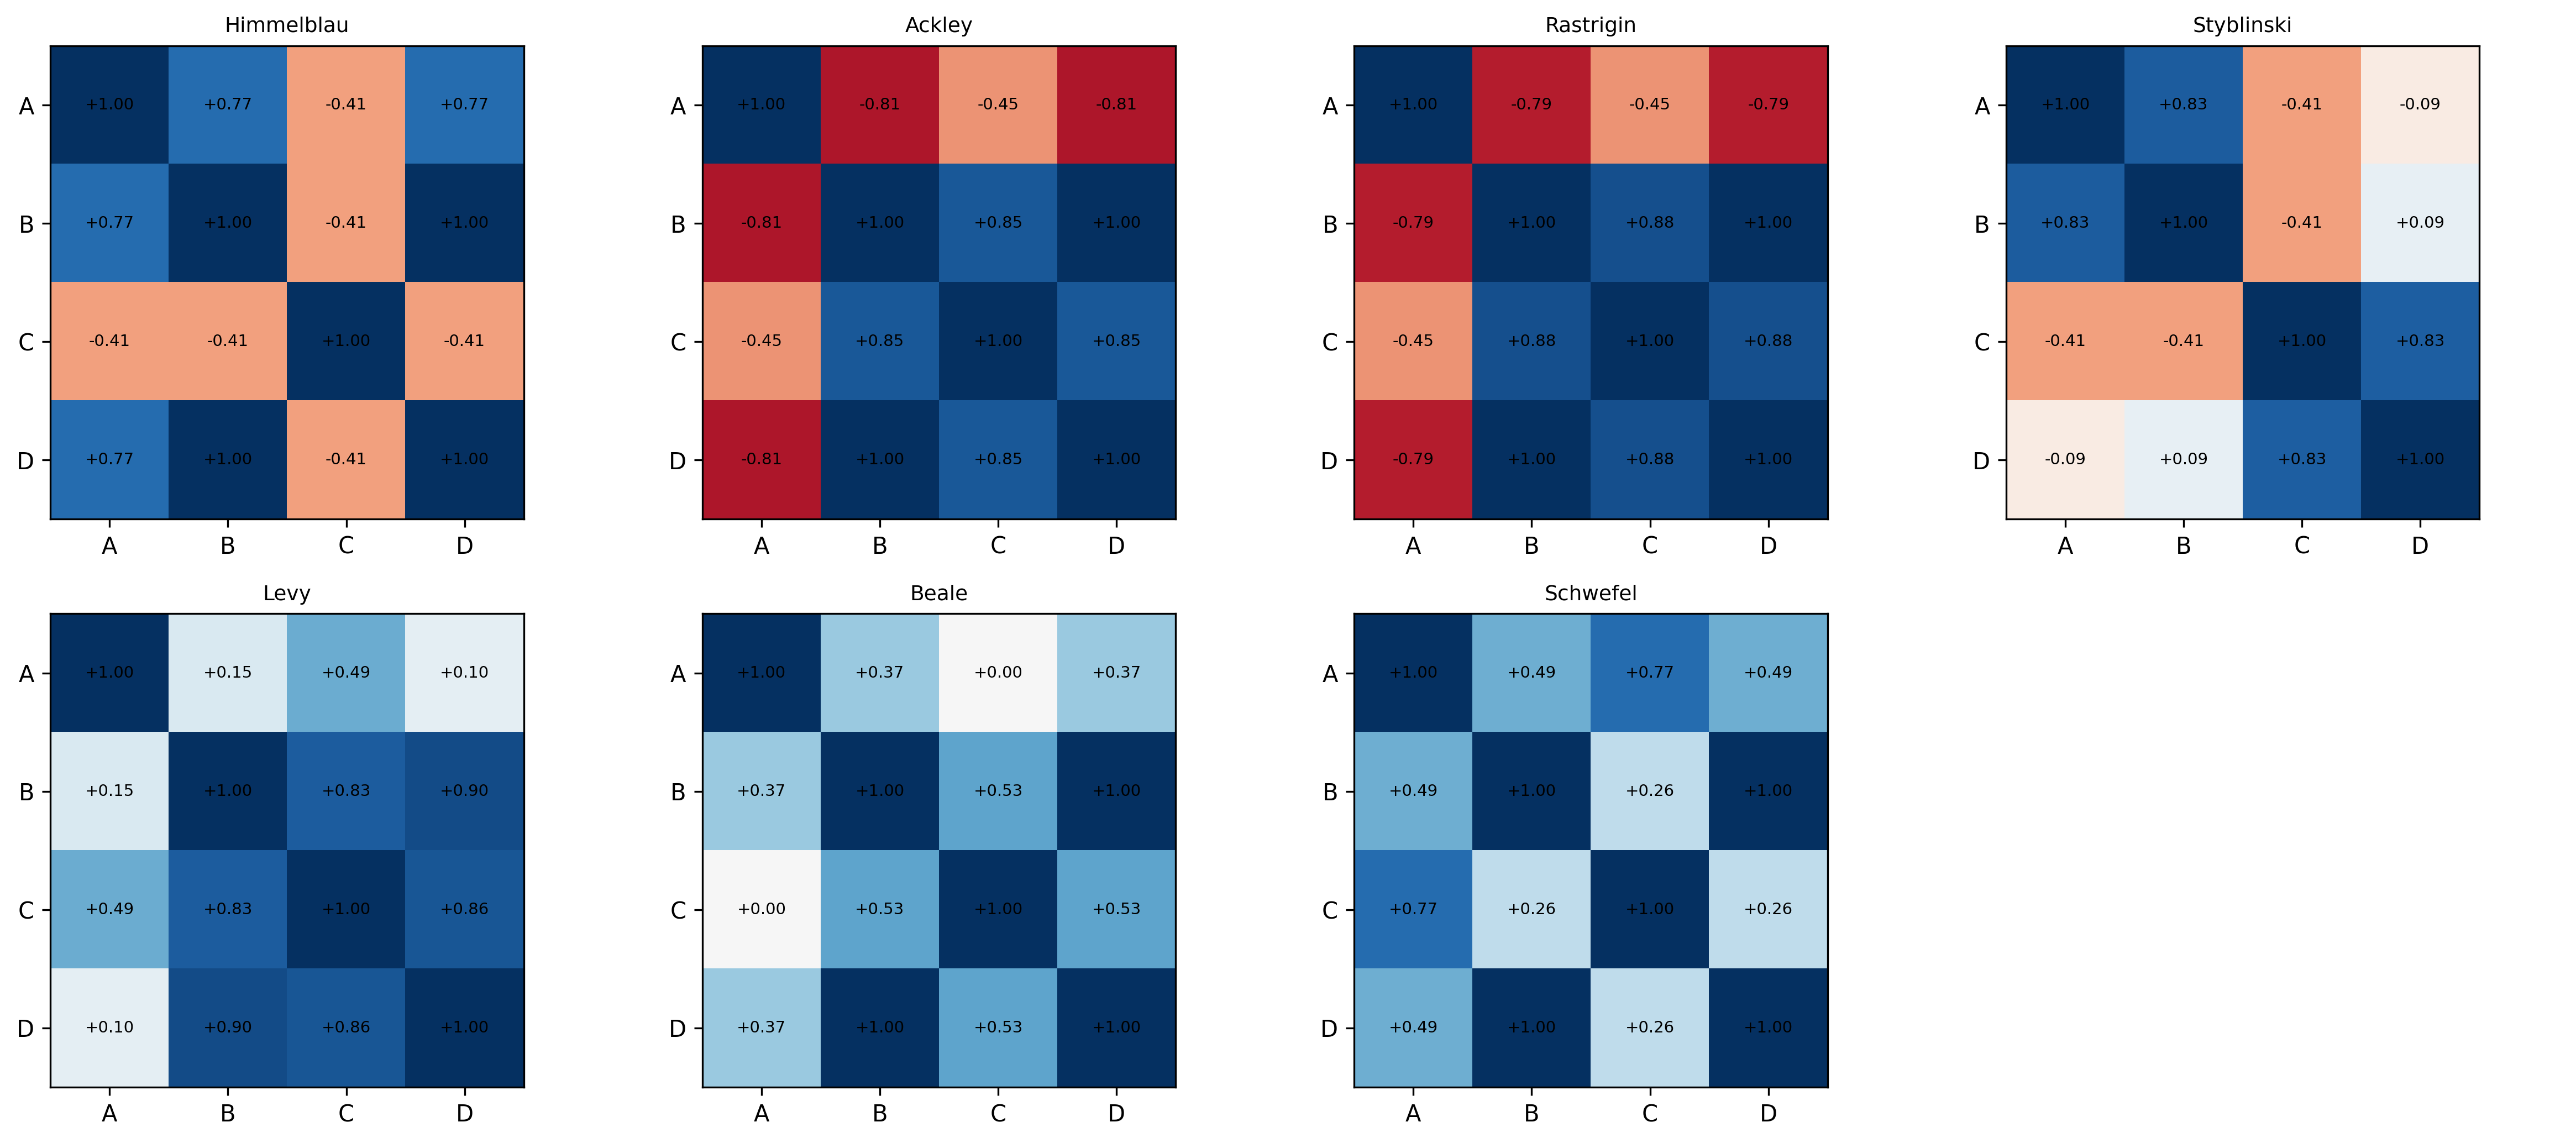
\includegraphics[width=0.95\textwidth]{../results/1_two_dimensional/figures/fig2_spearman.png}
\caption{Pairwise Spearman of best-LR SEE across criteria.}
\end{figure}

\begin{figure}[ht]\centering
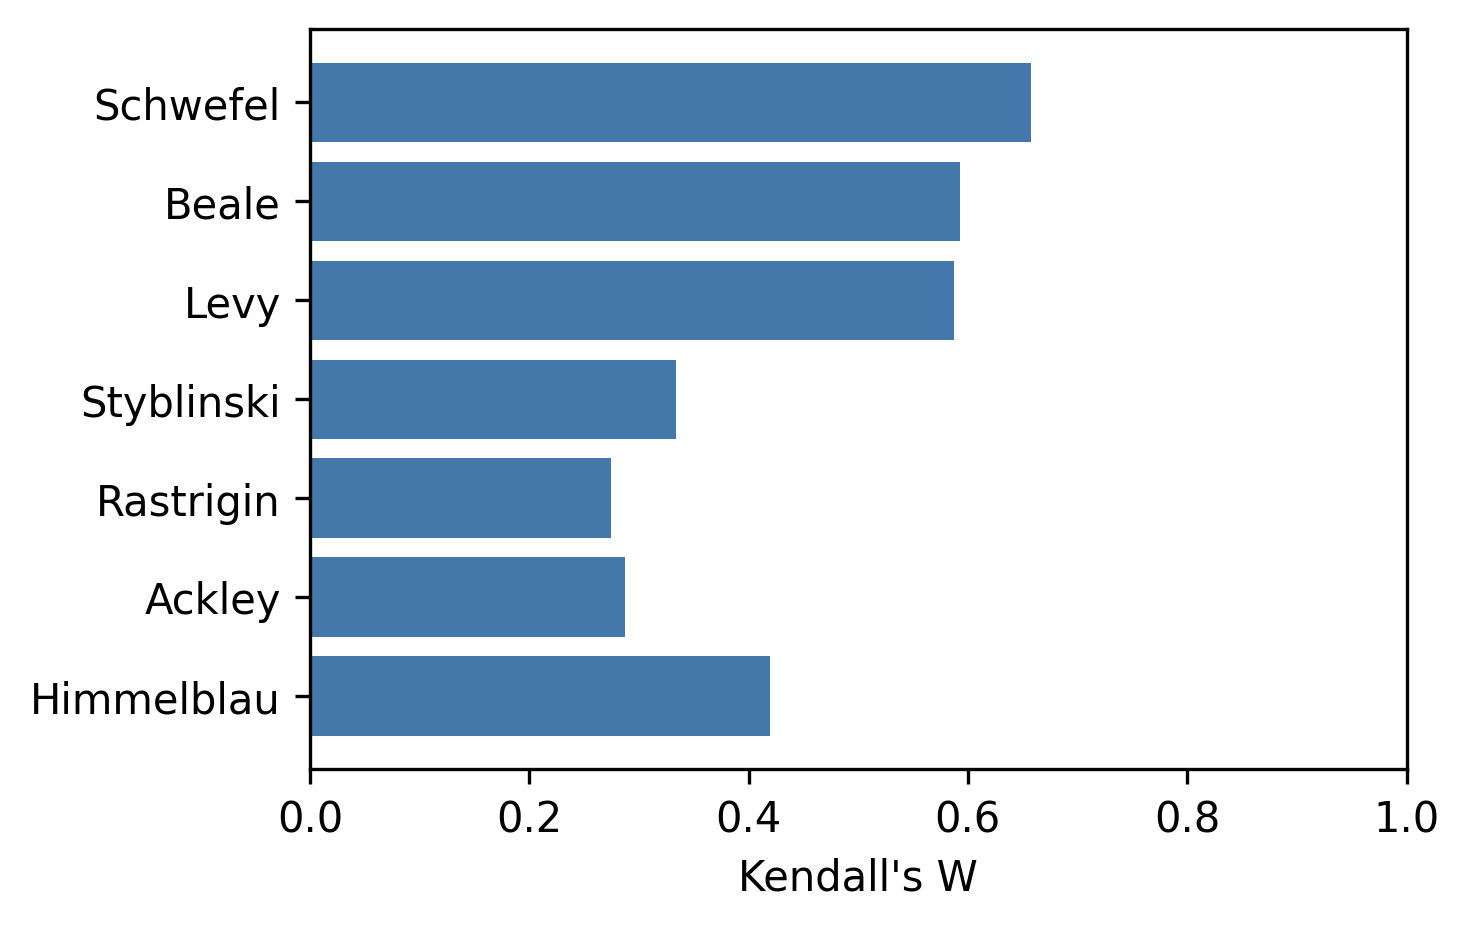
\includegraphics[width=0.55\textwidth]{../results/1_two_dimensional/figures/fig3_kendall_w.png}
\caption{Kendall's $W$ across A,B,C,D.}
\end{figure}

\begin{figure}[ht]\centering
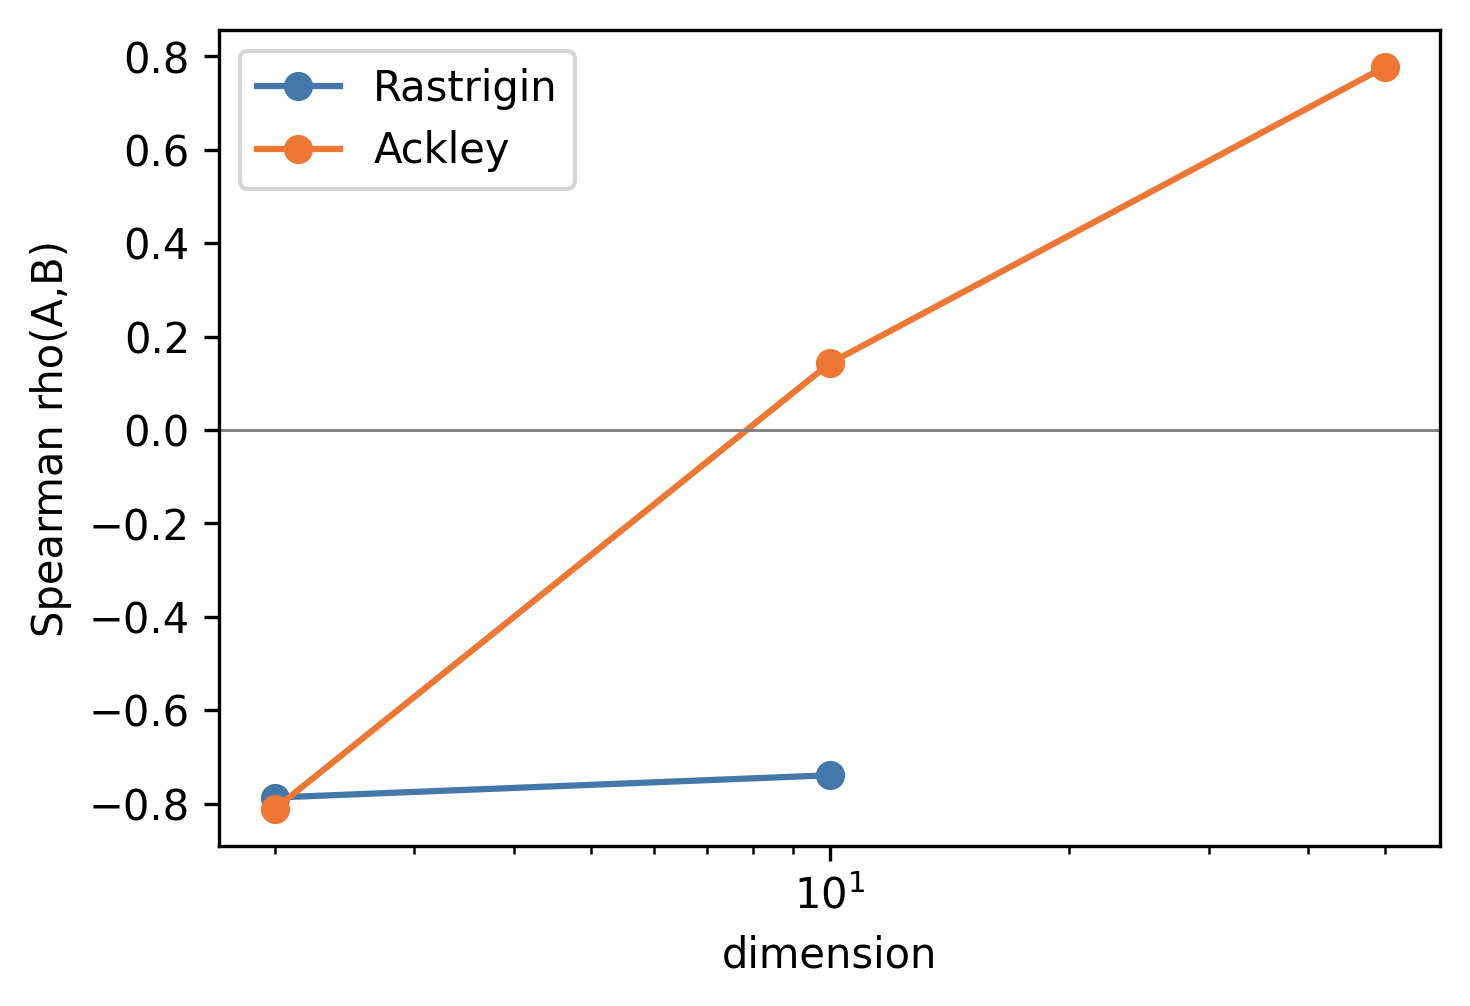
\includegraphics[width=0.55\textwidth]{../results/2_higher_dimension/figures/rho_ab_vs_dim.png}
\caption{Spearman $\rho(A,B)$ vs dimension (2D anchor from exp.~1).}
\end{figure}

\begin{figure}[ht]\centering
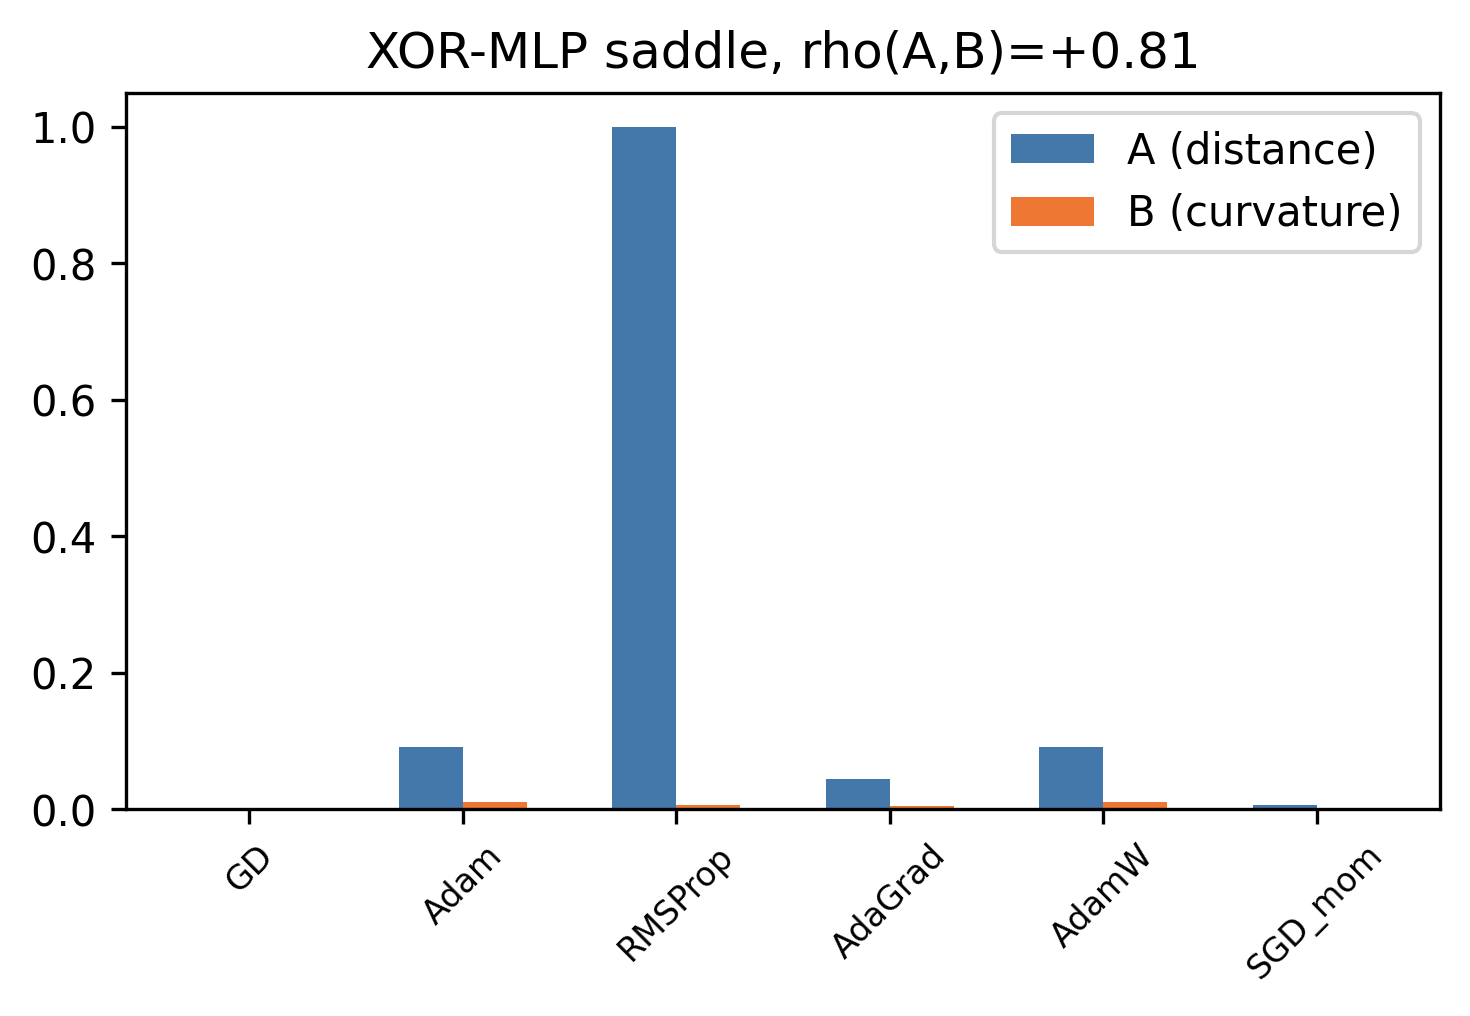
\includegraphics[width=0.55\textwidth]{../results/3_neural_network/figures/nn_AB.png}
\caption{XOR-MLP saddle, criteria A vs B.}
\end{figure}

\end{document}
